% % \section{Preliminaries}


% % \subsection{The Sequential Co-Design Pipeline}
% % \label{sec:background_pipeline}
% % % \begin{figure}[ht!]
% % %     \centering
% % %     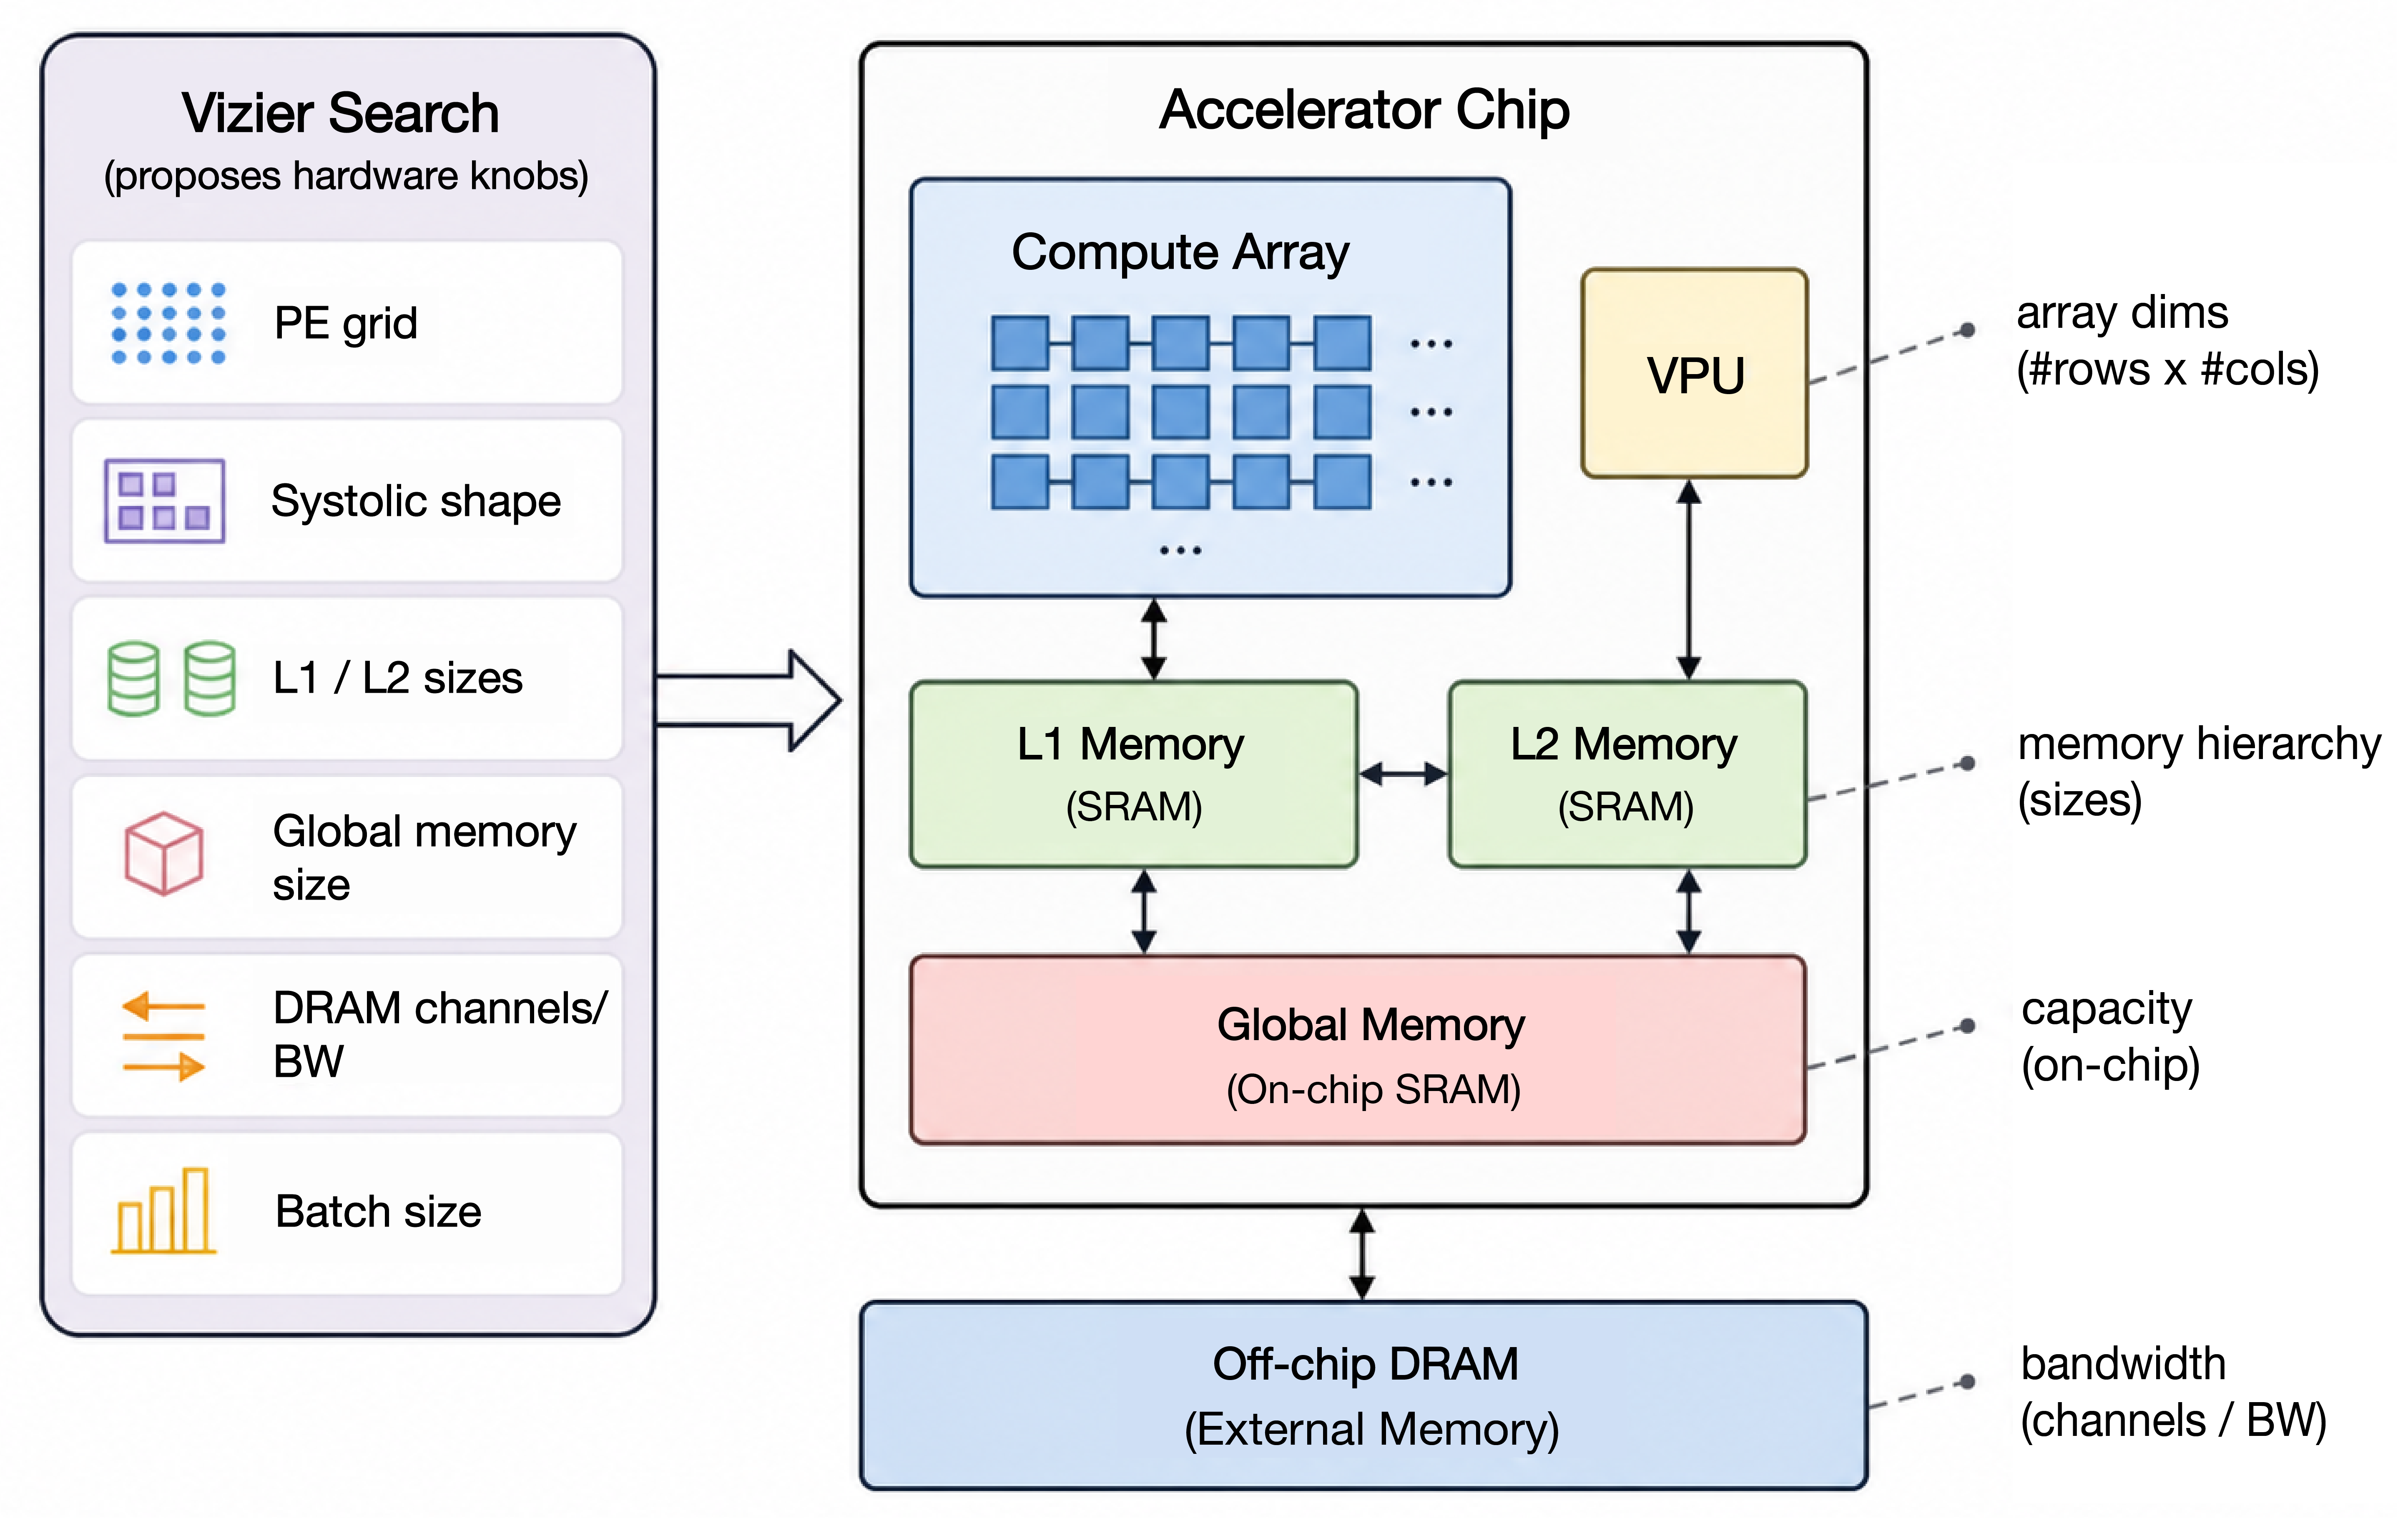
\includegraphics[width=0.7\linewidth]{figs/hardware_layout_v4.png}
% % %     \caption{The accelerator datapath configuration. Processing elements (PEs) are arranged in a grid connected by a mesh network. Each PE contains a systolic array for matrix operations, a vector processing unit (VPU) for non-MAC operations, and private or shared L1/L2 memory. A Global Memory serves as the on-chip scratchpad shared across all PEs.}
% % %     \label{fig:pipeline}
% % % \end{figure}
% % This section introduces FAST as our optimization framework baseline. The standard pipeline iterates for $\sim 5000$ times through three sequential stages: 
% % % We use the FAST accelerator template over PE grid, systolic dimensions, memory hierarchy, DRAM channels, and batch size.
% % % Section~\ref{sec:background_pipeline} provides background on the FAST sequential pipeline and identifies its limitations. 
% % % In Section \ref{sec:lps} we provide background on LPs and notation. FAST designs inference accelerators by iterating over three sequential stages:

% % \textbf{Stage 1: Hardware proposal.}
% % Vizier proposes a hardware configuration $\mathbf{h}$ consisting of 16 hyperparameters: PE grid dimensions, systolic array sizes, vector unit width, buffer configurations at L1/L2/Global levels, DRAM channels, and batch size. We defer a full picture of how Vizier's parameters specify a general accelerator chip template to Figure \ref{fig:pipeline} in the appendix.

% % % Figure \ref{fig:pipeline} shows how Vizier's parameters specify a general accelerator chip template. 
% % %The combined datapath search space is $\mathcal O(10^{13})$.

% % \textbf{Stage 2: Schedule optimization.}
% % For each operation $i$ in the neural network's XLA HLO graph, Timeloop finds the best tiling and mapping onto the hardware defined by $\mathbf{h}$. This produces execution time estimates $\Tmax_i$ (all tensors streamed from DRAM) and $\Tmin_i$ (all tensors on-chip), as well as per-tensor DRAM access costs $t_i^k$ for $k \in \{I, O, W\}$ (input activations, output activations, weights).

% % \textbf{Stage 3: Fusion ILP.}
% % Given fixed per-operation timing from Stage~2, an ILP decides which tensors to pin in the Global Memory to minimize total execution time. The ILP uses binary placement variables $p_i^k \in \{0,1\}$ indicating whether tensor $k$ of layer $i$ resides in Global Memory.

% % The result---predicted Perf/TDP---is returned to Vizier, which proposes the next $\mathbf{h}$. This repeats for ${\sim}5{,}000$ trials. See Appendix \ref{app:vizier} for details.

% % % \begin{table}[h]
% % % \centering
% % % \caption{Hardware configuration search space (Table 3 in FAST). All parameters are proposed by the outer-loop optimizer. In our \textcolor{skyblue}{V1} formulation, Global Buffer size can optionally be absorbed into the LP as described in Section~\ref{sec:v1}. \todo{change to the real range}}
% % % \label{tab:hw_params}
% % % \small
% % % \begin{tabular}{lll}
% % % \toprule
% % % \textbf{Parameter} & \textbf{Type} & \textbf{Range} \\
% % % \midrule
% % % PEs\_x\_dim, PEs\_y\_dim & int & 1--256, powers of 2 \\
% % % Systolic\_array\_x, Systolic\_array\_y & int & 1--256, powers of 2 \\
% % % Vector\_unit\_multiplier & int & 1--16, powers of 2 \\
% % % L1\_buffer\_config & enum & Private, Shared \\
% % % L1\_\{input,weight,output\}\_size & int & 1KB--1MB, powers of 2 \\
% % % L2\_buffer\_config & enum & Disabled, Private, Shared \\
% % % L2\_\{input,weight,output\}\_multiplier & int & 1$\times$--128$\times$, powers of 2 \\
% % % L3\_global\_buffer\_size & int & 0--256MB, powers of 2 \\
% % % GDDR6\_channels & int & 1--8, powers of 2 \\
% % % Native\_batch\_size & int & 1--256, powers of 2 \\
% % % \bottomrule
% % % \end{tabular}
% % % \end{table}

% % \paragraph{Sequential information loss limitation.}
% % Each stage commits to decisions that are irreversible by downstream stages. Timeloop optimizes each operation's tiling to minimize that operation's execution time \emph{in isolation}, without considering how tiling affects the feasibility or quality of fusion decisions. The fusion ILP receives fixed working-set sizes and cannot request alternative tiling configurations that might enable better global solutions. This sequential decomposition systematically misses trade-offs of the form: \emph{accept a tiling that reduces compute efficiency by $\delta$ but shrinks the working set enough to pin an additional tensor, removing a DRAM bottleneck worth $\gg \delta$}.

% % \subsection{Linear Programs and Solvers}
% % \label{sec:lps}
% % A Linear Program (LP) is a mathematical optimization technique for modeling systems of linear relationships. Formally, it consists of a linear objective function (such as minimizing a function of latency/throughput) subject to a set of linear inequality constraints that define a feasible solution region in a high-dimensional space. However the relationship between tiling, fusion, and memory is often non-linear, which restricts the expressiveness of the problem formulation. We list this restriction by utilizing McCormick envelopes to provide a tight relaxation, ensuring that the gap between the continuous LP "ideal" and the final rounded hardware spec remains minimal. This enables CHEETAH to capture globally optimal solutions without sacrificing optimality due to restrictive linear/scale limitations.

% % page edit

% \section{Preliminaries}


% \subsection{The Sequential Co-Design Pipeline}
% \label{sec:background_pipeline}
% % \begin{figure}[ht!]
% %     \centering
% %     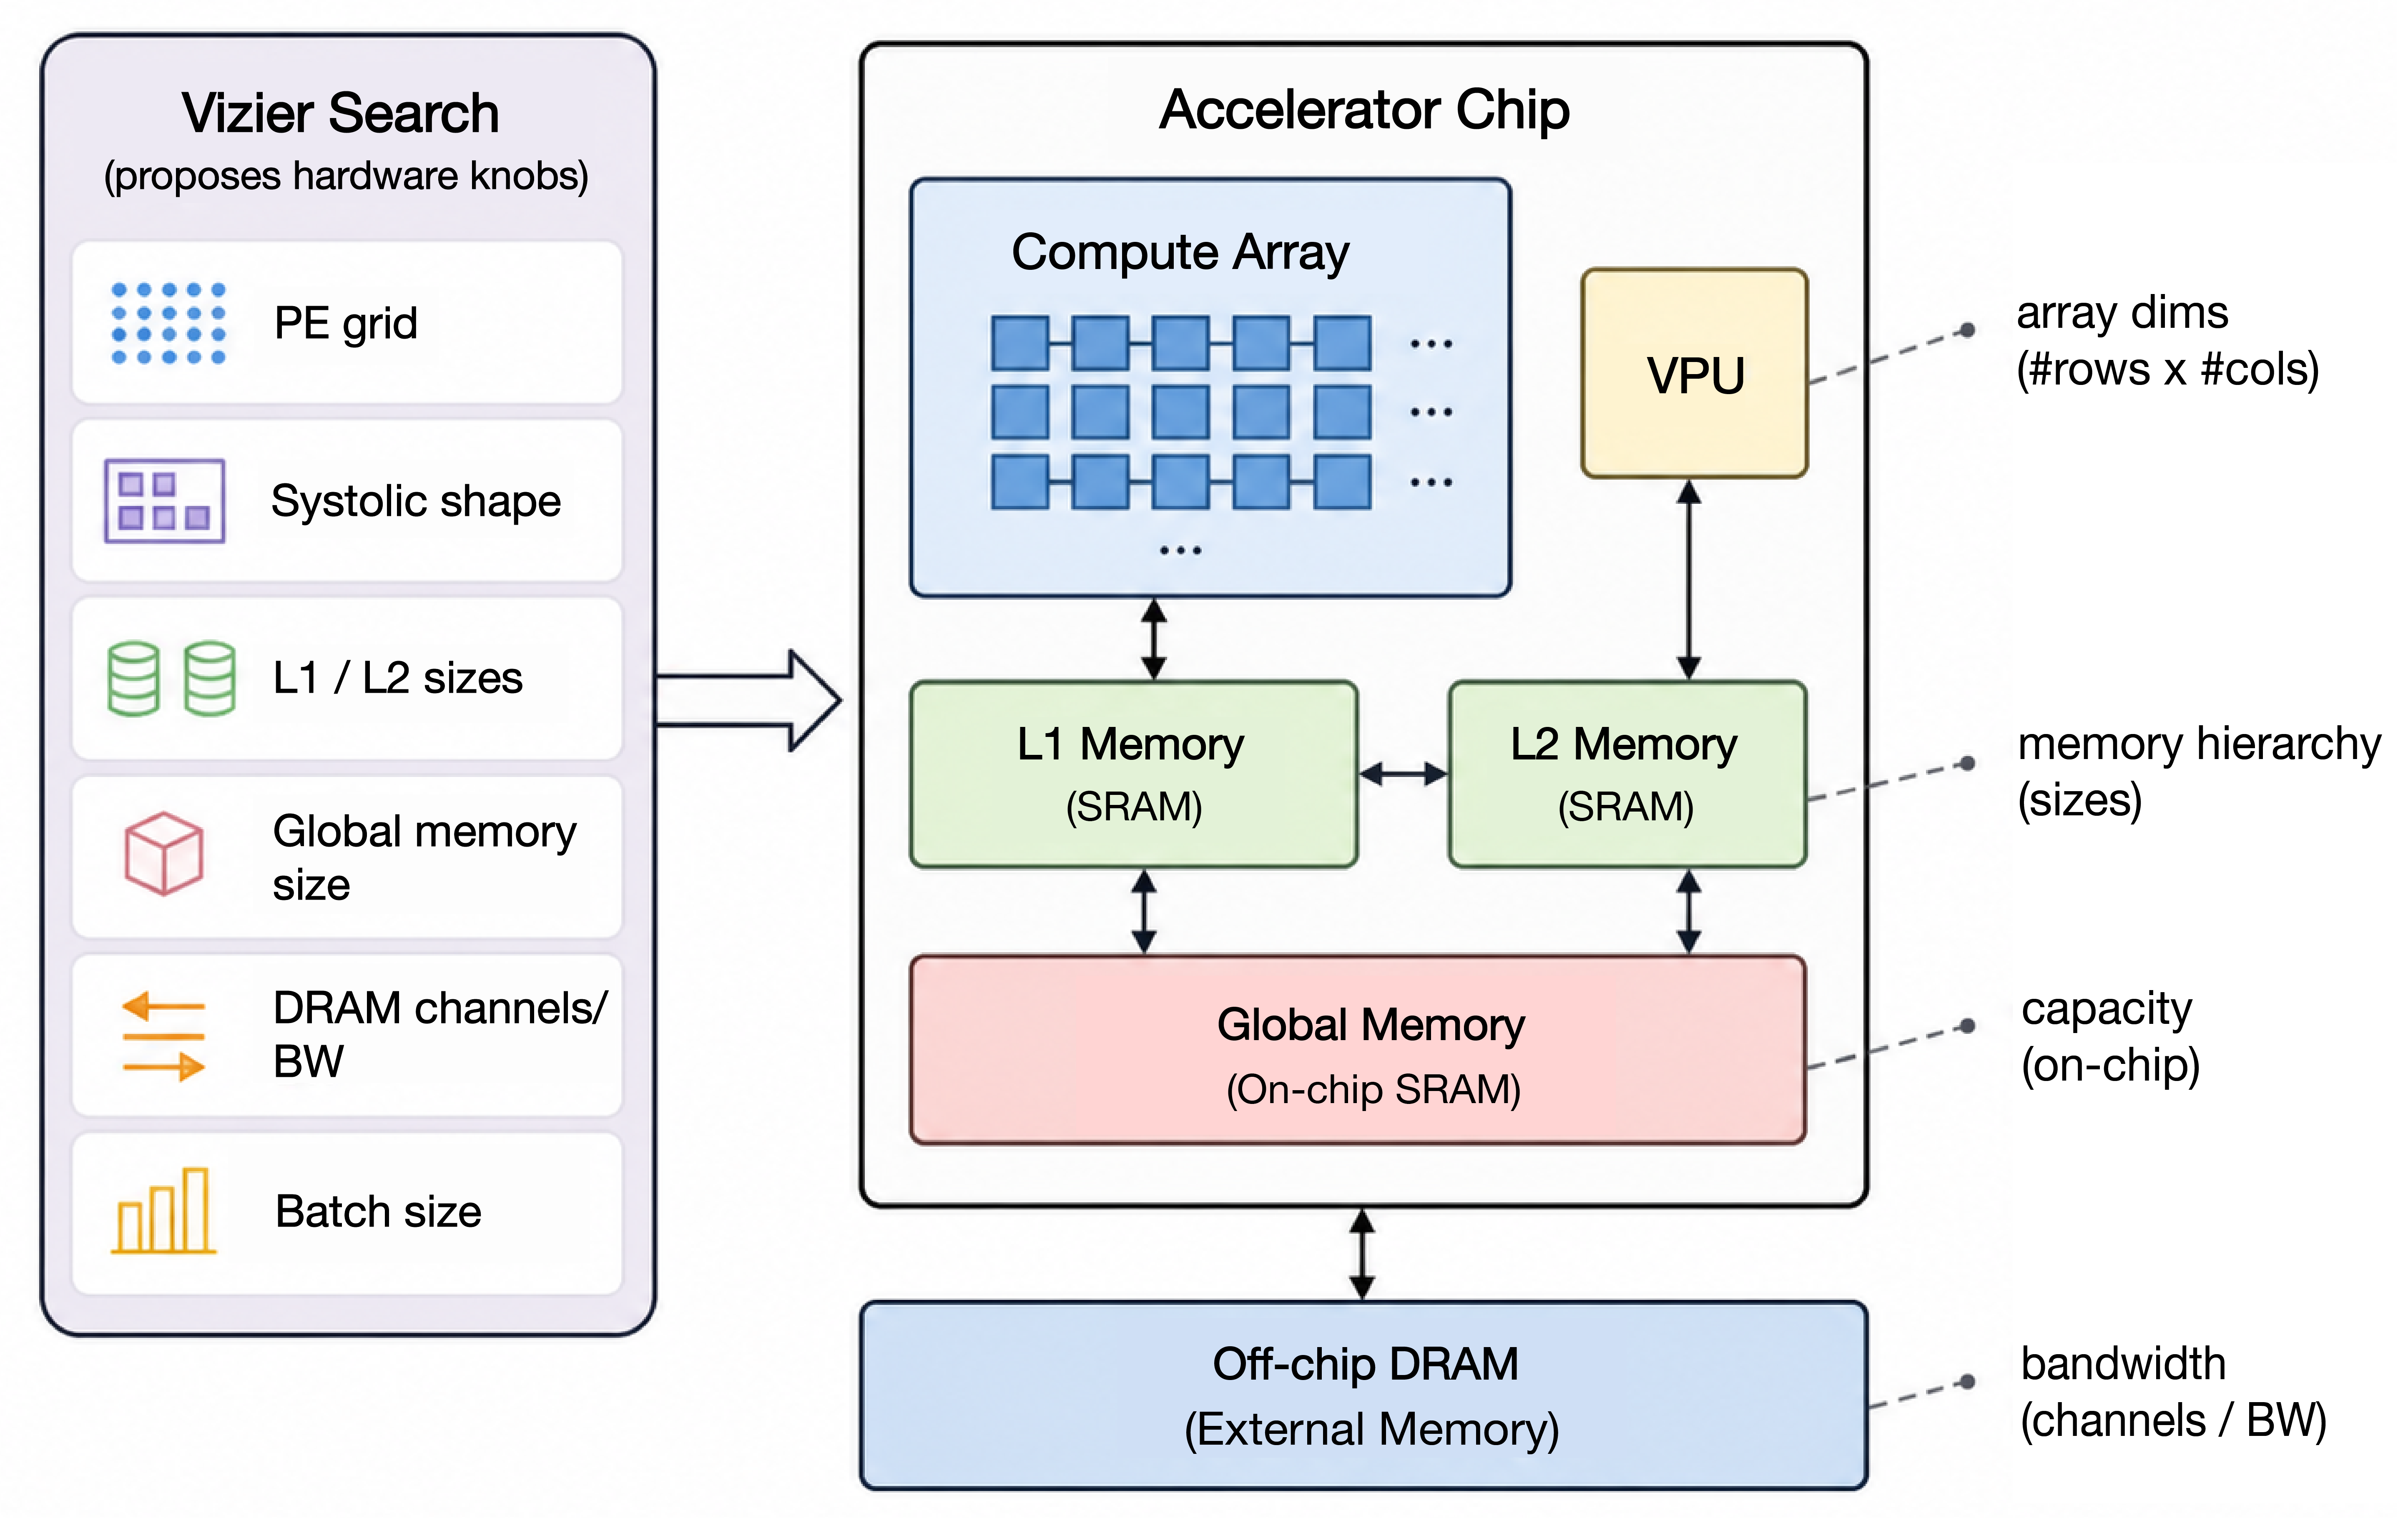
\includegraphics[width=0.7\linewidth]{figs/hardware_layout_v4.png}
% %     \caption{The accelerator datapath configuration. Processing elements (PEs) are arranged in a grid connected by a mesh network. Each PE contains a systolic array for matrix operations, a vector processing unit (VPU) for non-MAC operations, and private or shared L1/L2 memory. A Global Memory serves as the on-chip scratchpad shared across all PEs.}
% %     \label{fig:pipeline}
% % \end{figure}
% This section introduces FAST as our optimization framework baseline. The standard pipeline iterates for $\sim 5000$ times through three sequential stages: 
% % We use the FAST accelerator template over PE grid, systolic dimensions, memory hierarchy, DRAM channels, and batch size.
% % Section~\ref{sec:background_pipeline} provides background on the FAST sequential pipeline and identifies its limitations. 
% % In Section \ref{sec:lps} we provide background on LPs and notation. FAST designs inference accelerators by iterating over three sequential stages:

% \textbf{Stage 1: Hardware proposal.}
% Vizier proposes a hardware configuration $\mathbf{h}$ consisting of 16 hyperparameters: PE grid dimensions, systolic array sizes, vector unit width, buffer configurations at L1/L2/Global levels, DRAM channels, and batch size. We defer a full picture of how Vizier's parameters specify a general accelerator chip template to Figure \ref{fig:pipeline} in the appendix.

% % Figure \ref{fig:pipeline} shows how Vizier's parameters specify a general accelerator chip template. 
% %The combined datapath search space is $\mathcal O(10^{13})$.

% \textbf{Stage 2: Schedule optimization.}
% For each operation $i$ in the neural network's XLA HLO graph, Timeloop finds the best tiling and mapping onto the hardware defined by $\mathbf{h}$. This produces execution time estimates $\Tmax_i$ (all tensors streamed from DRAM) and $\Tmin_i$ (all tensors on-chip), as well as per-tensor DRAM access costs $t_i^k$ for $k \in \{I, O, W\}$ (input activations, output activations, weights).

% \textbf{Stage 3: Fusion ILP.}
% Given fixed per-operation timing from Stage~2, an ILP decides which tensors to pin in the Global Memory to minimize total execution time. The ILP uses binary placement variables $p_i^k \in \{0,1\}$ indicating whether tensor $k$ of layer $i$ resides in Global Memory.

% The result---predicted Perf/TDP---is returned to Vizier, which proposes the next $\mathbf{h}$. This repeats for ${\sim}5{,}000$ trials. See Appendix \ref{app:vizier} for details.

% % \begin{table}[h]
% % \centering
% % \caption{Hardware configuration search space (Table 3 in FAST). All parameters are proposed by the outer-loop optimizer. In our \textcolor{skyblue}{V1} formulation, Global Buffer size can optionally be absorbed into the LP as described in Section~\ref{sec:v1}. \todo{change to the real range}}
% % \label{tab:hw_params}
% % \small
% % \begin{tabular}{lll}
% % \toprule
% % \textbf{Parameter} & \textbf{Type} & \textbf{Range} \\
% % \midrule
% % PEs\_x\_dim, PEs\_y\_dim & int & 1--256, powers of 2 \\
% % Systolic\_array\_x, Systolic\_array\_y & int & 1--256, powers of 2 \\
% % Vector\_unit\_multiplier & int & 1--16, powers of 2 \\
% % L1\_buffer\_config & enum & Private, Shared \\
% % L1\_\{input,weight,output\}\_size & int & 1KB--1MB, powers of 2 \\
% % L2\_buffer\_config & enum & Disabled, Private, Shared \\
% % L2\_\{input,weight,output\}\_multiplier & int & 1$\times$--128$\times$, powers of 2 \\
% % L3\_global\_buffer\_size & int & 0--256MB, powers of 2 \\
% % GDDR6\_channels & int & 1--8, powers of 2 \\
% % Native\_batch\_size & int & 1--256, powers of 2 \\
% % \bottomrule
% % \end{tabular}
% % \end{table}

% \paragraph{Limitations and sequential information loss.}
% Each stage commits to decisions that are irreversible by downstream stages. Timeloop optimizes each operation's tiling to minimize that operation's execution time \emph{in isolation}, without considering how tiling affects the feasibility or quality of fusion decisions. The fusion ILP receives fixed working-set sizes and cannot request alternative tiling configurations that might enable better global solutions. This sequential decomposition systematically misses trade-offs of the form: \emph{accept a tiling that reduces compute efficiency by $\delta$ but shrinks the working set enough to pin an additional tensor, removing a DRAM bottleneck worth $\gg \delta$}.

% \vspace{-6pt}
% \subsection{Linear Programs and Solvers}
% \label{sec:lps}
% Standard LPs cannot directly express the nonlinear interaction between tiling, fusion, and memory. We address this via McCormick envelopes~\citep{mccormick1976computability}, which provide a tight convex relaxation of bilinear terms, ensuring that the gap between the continuous LP solution and the final rounded hardware specification remains minimal.


% page limit edit

% \section{Preliminaries}


% \subsection{The Sequential Co-Design Pipeline}
% \label{sec:background_pipeline}
% % \begin{figure}[ht!]
% %     \centering
% %     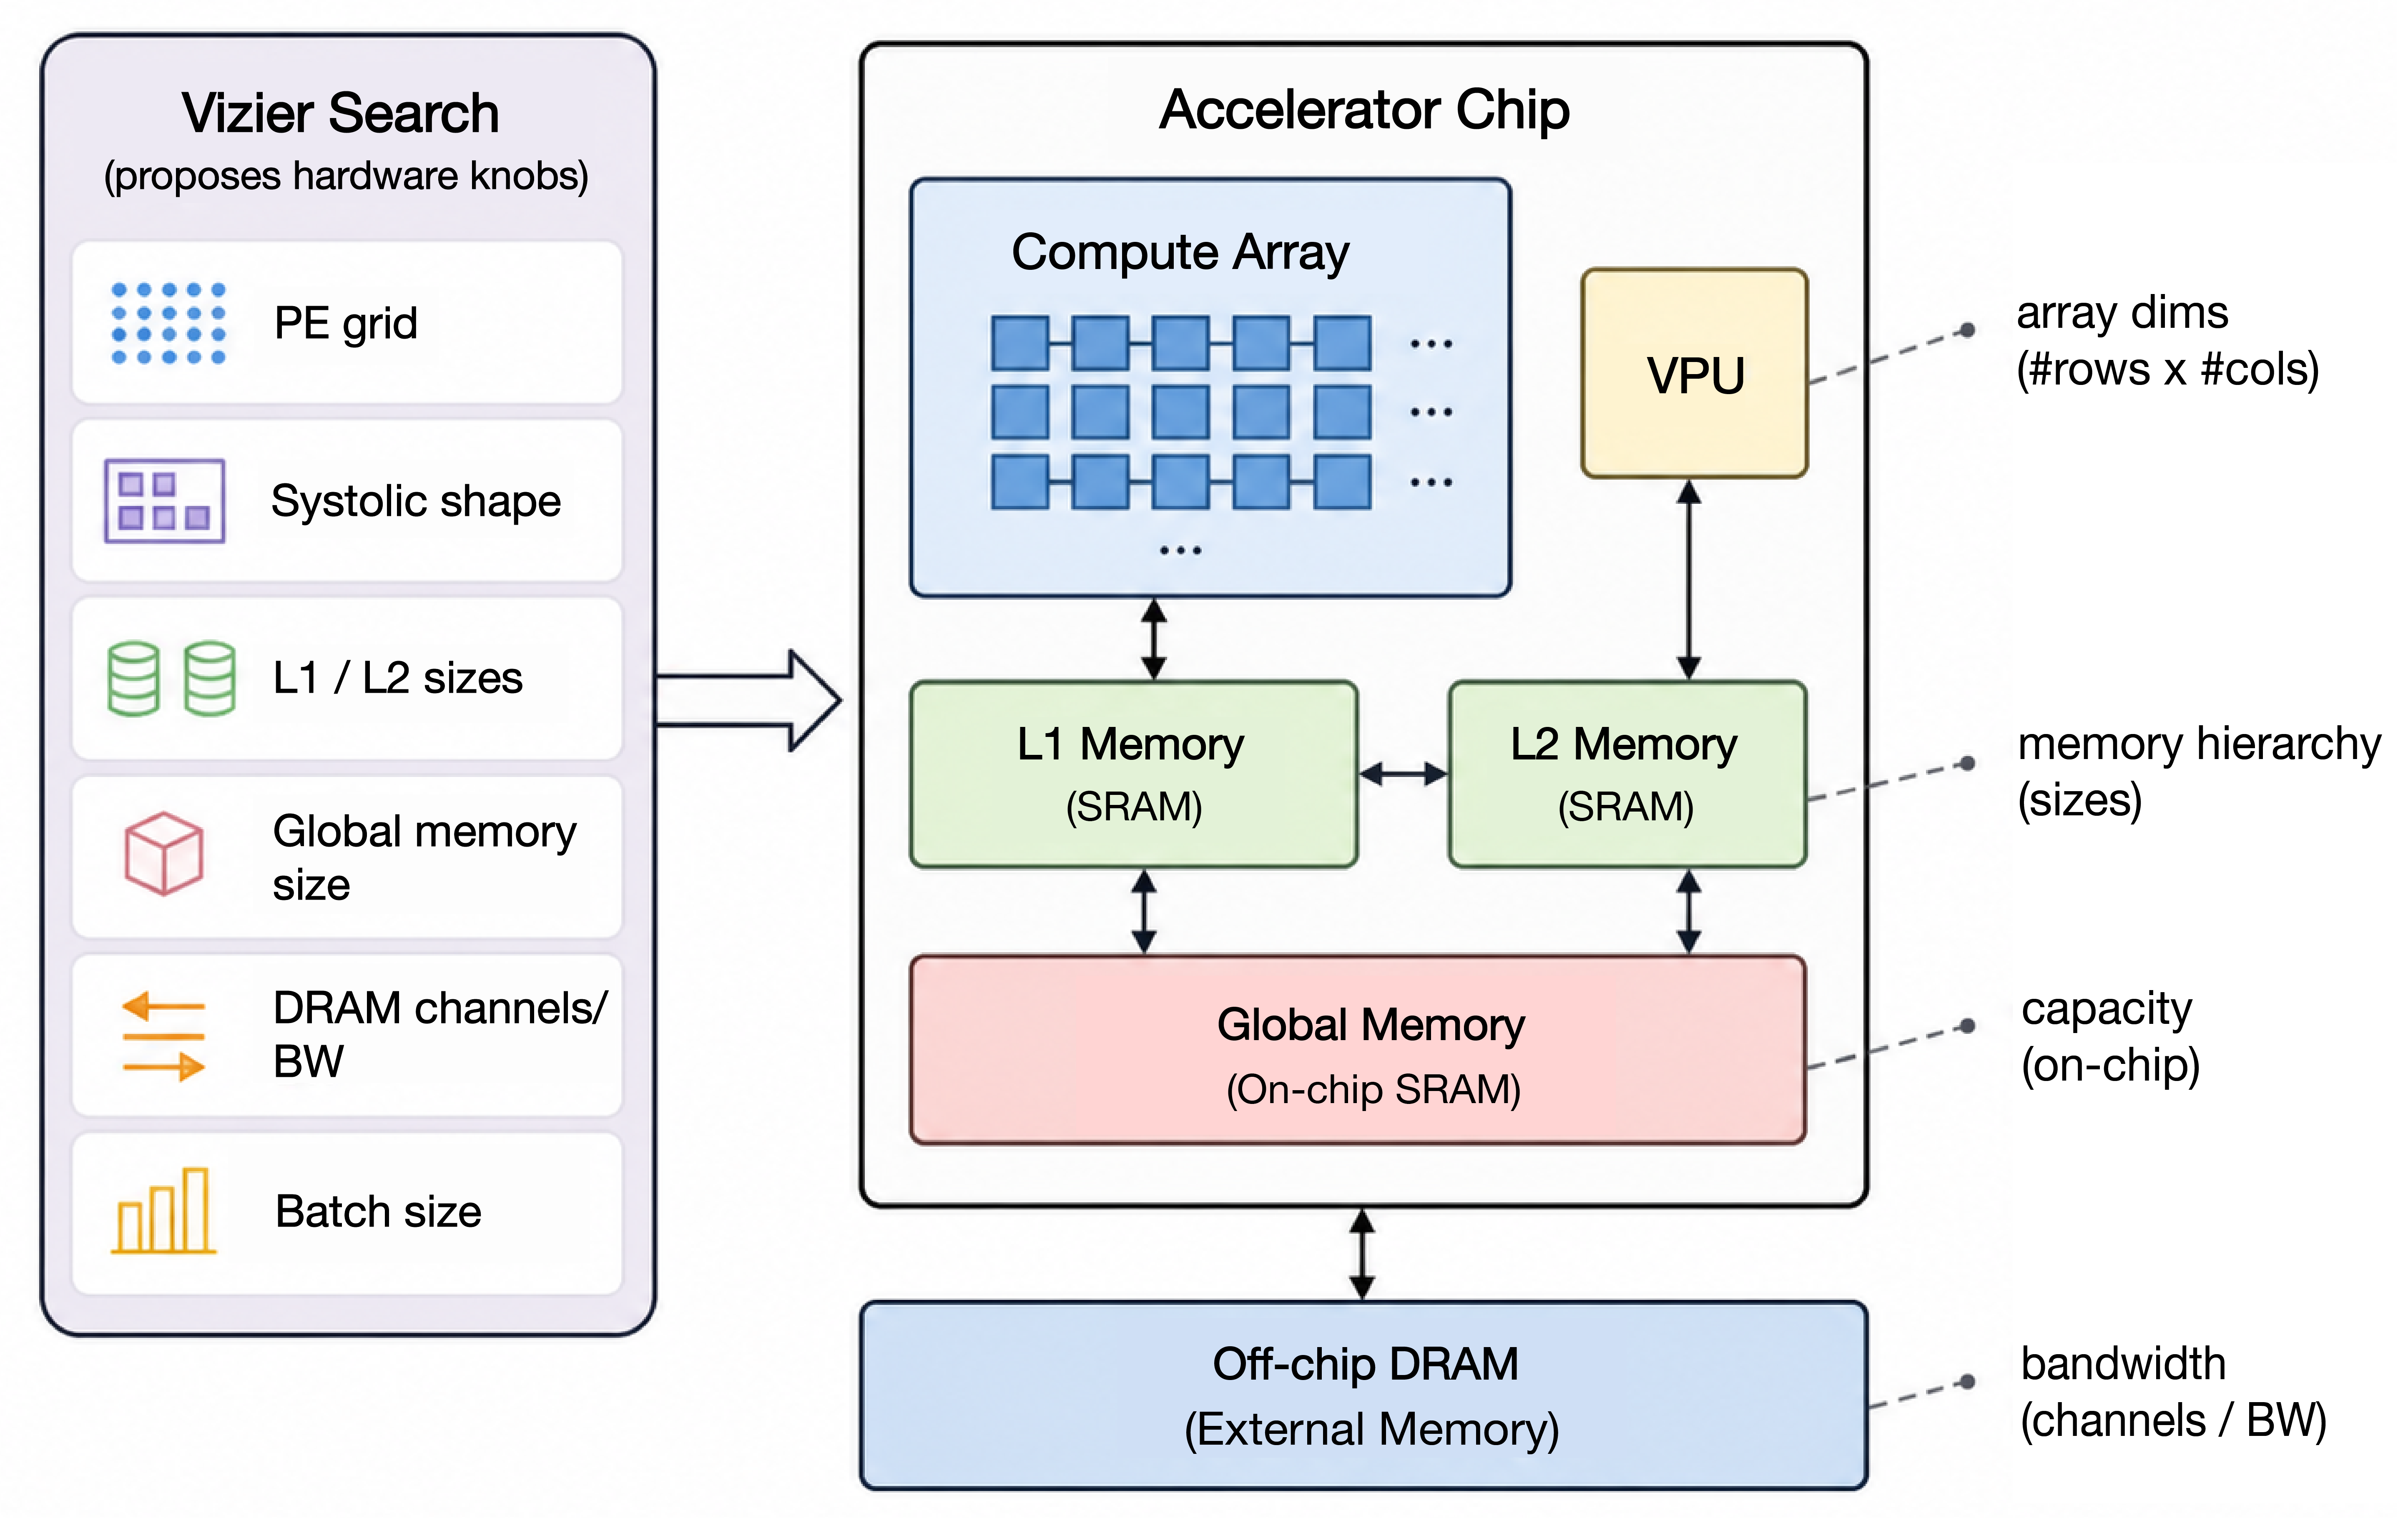
\includegraphics[width=0.7\linewidth]{figs/hardware_layout_v4.png}
% %     \caption{The accelerator datapath configuration. Processing elements (PEs) are arranged in a grid connected by a mesh network. Each PE contains a systolic array for matrix operations, a vector processing unit (VPU) for non-MAC operations, and private or shared L1/L2 memory. A Global Memory serves as the on-chip scratchpad shared across all PEs.}
% %     \label{fig:pipeline}
% % \end{figure}
% This section introduces FAST as our optimization framework baseline. The standard pipeline iterates for $\sim 5000$ times through three sequential stages: 
% % We use the FAST accelerator template over PE grid, systolic dimensions, memory hierarchy, DRAM channels, and batch size.
% % Section~\ref{sec:background_pipeline} provides background on the FAST sequential pipeline and identifies its limitations. 
% % In Section \ref{sec:lps} we provide background on LPs and notation. FAST designs inference accelerators by iterating over three sequential stages:

% \textbf{Stage 1: Hardware proposal.}
% Vizier proposes a hardware configuration $\mathbf{h}$ consisting of 16 hyperparameters: PE grid dimensions, systolic array sizes, vector unit width, buffer configurations at L1/L2/Global levels, DRAM channels, and batch size. We defer a full picture of how Vizier's parameters specify a general accelerator chip template to Figure \ref{fig:pipeline} in the appendix.

% % Figure \ref{fig:pipeline} shows how Vizier's parameters specify a general accelerator chip template. 
% %The combined datapath search space is $\mathcal O(10^{13})$.

% \textbf{Stage 2: Schedule optimization.}
% For each operation $i$ in the neural network's XLA HLO graph, Timeloop finds the best tiling and mapping onto the hardware defined by $\mathbf{h}$. This produces execution time estimates $\Tmax_i$ (all tensors streamed from DRAM) and $\Tmin_i$ (all tensors on-chip), as well as per-tensor DRAM access costs $t_i^k$ for $k \in \{I, O, W\}$ (input activations, output activations, weights).

% \textbf{Stage 3: Fusion ILP.}
% Given fixed per-operation timing from Stage~2, an ILP decides which tensors to pin in the Global Memory to minimize total execution time. The ILP uses binary placement variables $p_i^k \in \{0,1\}$ indicating whether tensor $k$ of layer $i$ resides in Global Memory.

% The result---predicted Perf/TDP---is returned to Vizier, which proposes the next $\mathbf{h}$. This repeats for ${\sim}5{,}000$ trials. See Appendix \ref{app:vizier} for details.

% % \begin{table}[h]
% % \centering
% % \caption{Hardware configuration search space (Table 3 in FAST). All parameters are proposed by the outer-loop optimizer. In our \textcolor{skyblue}{V1} formulation, Global Buffer size can optionally be absorbed into the LP as described in Section~\ref{sec:v1}. \todo{change to the real range}}
% % \label{tab:hw_params}
% % \small
% % \begin{tabular}{lll}
% % \toprule
% % \textbf{Parameter} & \textbf{Type} & \textbf{Range} \\
% % \midrule
% % PEs\_x\_dim, PEs\_y\_dim & int & 1--256, powers of 2 \\
% % Systolic\_array\_x, Systolic\_array\_y & int & 1--256, powers of 2 \\
% % Vector\_unit\_multiplier & int & 1--16, powers of 2 \\
% % L1\_buffer\_config & enum & Private, Shared \\
% % L1\_\{input,weight,output\}\_size & int & 1KB--1MB, powers of 2 \\
% % L2\_buffer\_config & enum & Disabled, Private, Shared \\
% % L2\_\{input,weight,output\}\_multiplier & int & 1$\times$--128$\times$, powers of 2 \\
% % L3\_global\_buffer\_size & int & 0--256MB, powers of 2 \\
% % GDDR6\_channels & int & 1--8, powers of 2 \\
% % Native\_batch\_size & int & 1--256, powers of 2 \\
% % \bottomrule
% % \end{tabular}
% % \end{table}

% \paragraph{Sequential information loss limitation.}
% Each stage commits to decisions that are irreversible by downstream stages. Timeloop optimizes each operation's tiling to minimize that operation's execution time \emph{in isolation}, without considering how tiling affects the feasibility or quality of fusion decisions. The fusion ILP receives fixed working-set sizes and cannot request alternative tiling configurations that might enable better global solutions. This sequential decomposition systematically misses trade-offs of the form: \emph{accept a tiling that reduces compute efficiency by $\delta$ but shrinks the working set enough to pin an additional tensor, removing a DRAM bottleneck worth $\gg \delta$}.

% \subsection{Linear Programs and Solvers}
% \label{sec:lps}
% A Linear Program (LP) is a mathematical optimization technique for modeling systems of linear relationships. Formally, it consists of a linear objective function (such as minimizing a function of latency/throughput) subject to a set of linear inequality constraints that define a feasible solution region in a high-dimensional space. However the relationship between tiling, fusion, and memory is often non-linear, which restricts the expressiveness of the problem formulation. We list this restriction by utilizing McCormick envelopes to provide a tight relaxation, ensuring that the gap between the continuous LP "ideal" and the final rounded hardware spec remains minimal. This enables CHEETAH to capture globally optimal solutions without sacrificing optimality due to restrictive linear/scale limitations.

% page edit

\section{Preliminaries}
This section provides background and defines notation. \cref{sec:background_pipeline} outlines the HW/SW co-design problem, and \cref{sec:lps} introduces the setting for linear programs and their large-scale solvers.

\subsection{The Sequential Co-Design Pipeline}
\label{sec:background_pipeline}
% \begin{figure}[ht!]
%     \centering
%     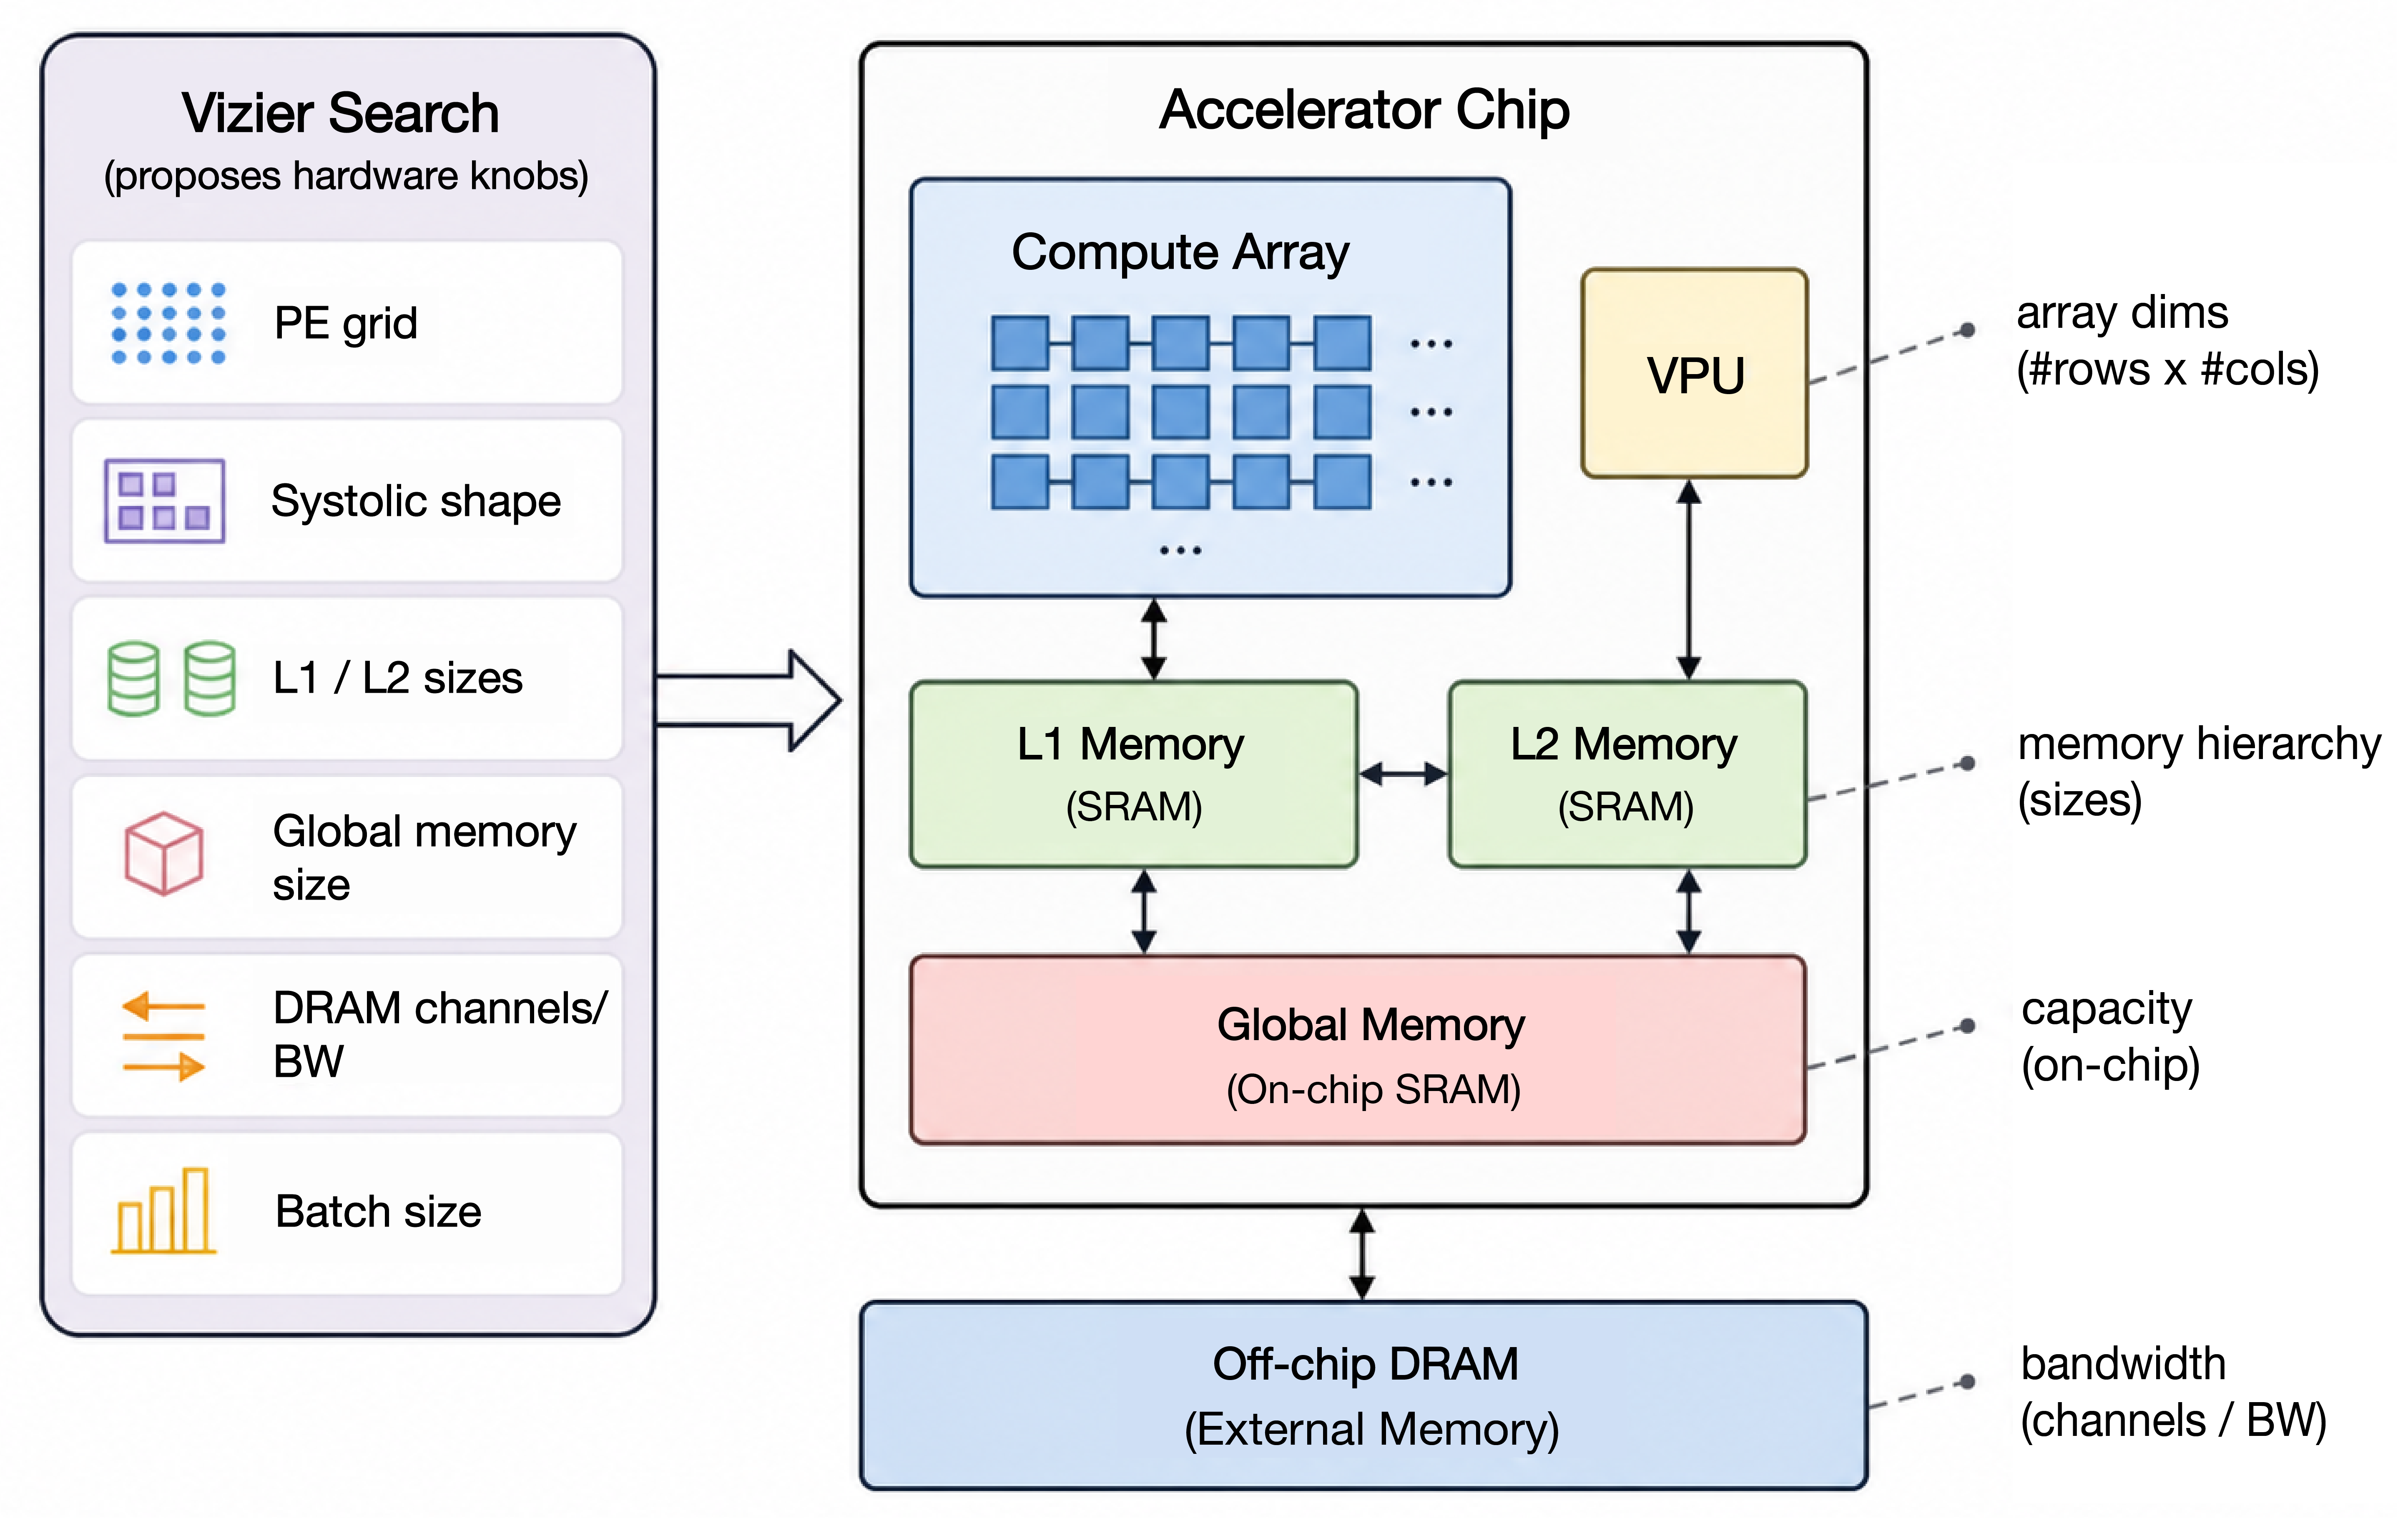
\includegraphics[width=0.7\linewidth]{figs/hardware_layout_v4.png}
%     \caption{The accelerator datapath configuration. Processing elements (PEs) are arranged in a grid connected by a mesh network. Each PE contains a systolic array for matrix operations, a vector processing unit (VPU) for non-MAC operations, and private or shared L1/L2 memory. A Global Memory serves as the on-chip scratchpad shared across all PEs.}
%     \label{fig:pipeline}
% \end{figure}
The standard pipeline iterates for a minimum of $\sim 5000$ times through three sequential stages: 
% We use the FAST accelerator template over PE grid, systolic dimensions, memory hierarchy, DRAM channels, and batch size.
% Section~\ref{sec:background_pipeline} provides background on the FAST sequential pipeline and identifies its limitations. 
% In Section \ref{sec:lps} we provide background on LPs and notation. FAST designs inference accelerators by iterating over three sequential stages:

\textbf{Stage 1: Hardware proposal.}
Vizier proposes a hardware configuration $\mathbf{h}$ consisting of 16 hyperparameters: PE grid dimensions, systolic array sizes, vector unit width, buffer configurations at L1/L2/Global levels, DRAM channels, and batch size. We defer a full picture of how Vizier's parameters specify a general accelerator chip template to Figure \ref{fig:pipeline} in the appendix.

% Figure \ref{fig:pipeline} shows how Vizier's parameters specify a general accelerator chip template. 
%The combined datapath search space is $\mathcal O(10^{13})$.

\textbf{Stage 2: Schedule optimization.}
For each operation $i$ in the neural network's XLA HLO graph, Timeloop finds the best tiling and mapping onto the hardware defined by $\mathbf{h}$. This produces execution time estimates $\Tmax_i$ (all tensors streamed from DRAM) and $\Tmin_i$ (all tensors on-chip), as well as per-tensor DRAM access costs $t_i^k$ for $k \in \{I, O, W\}$ (input activations, output activations, weights).

\textbf{Stage 3: Fusion ILP.}
Given fixed per-operation timing from Stage~2, an ILP decides which tensors to pin in the Global Memory to minimize total execution time. The ILP uses binary placement variables $p_i^k \in \{0,1\}$ indicating whether tensor $k$ of layer $i$ resides in Global Memory.

The result (predicted Perf/TDP) is returned to Vizier, which proposes the next $\mathbf{h}$. This repeats for ${\sim}5{,}000$ trials. See Appendix \ref{app:vizier} for details.

% \begin{table}[h]
% \centering
% \caption{Hardware configuration search space (Table 3 in FAST). All parameters are proposed by the outer-loop optimizer. In our \textcolor{skyblue}{V1} formulation, Global Buffer size can optionally be absorbed into the LP as described in Section~\ref{sec:v1}. \todo{change to the real range}}
% \label{tab:hw_params}
% \small
% \begin{tabular}{lll}
% \toprule
% \textbf{Parameter} & \textbf{Type} & \textbf{Range} \\
% \midrule
% PEs\_x\_dim, PEs\_y\_dim & int & 1--256, powers of 2 \\
% Systolic\_array\_x, Systolic\_array\_y & int & 1--256, powers of 2 \\
% Vector\_unit\_multiplier & int & 1--16, powers of 2 \\
% L1\_buffer\_config & enum & Private, Shared \\
% L1\_\{input,weight,output\}\_size & int & 1KB--1MB, powers of 2 \\
% L2\_buffer\_config & enum & Disabled, Private, Shared \\
% L2\_\{input,weight,output\}\_multiplier & int & 1$\times$--128$\times$, powers of 2 \\
% L3\_global\_buffer\_size & int & 0--256MB, powers of 2 \\
% GDDR6\_channels & int & 1--8, powers of 2 \\
% Native\_batch\_size & int & 1--256, powers of 2 \\
% \bottomrule
% \end{tabular}
% \end{table}

\paragraph{Limitations and sequential information loss.}
Each stage commits to decisions that are irreversible by downstream stages. Timeloop optimizes each operation's tiling to minimize that operation's execution time \emph{in isolation}, without considering how tiling affects the feasibility or quality of fusion decisions. The fusion ILP receives fixed working-set sizes and cannot request alternative tiling configurations that might enable better global solutions. This sequential decomposition systematically misses trade-offs of the form: \emph{accept a tiling that reduces compute efficiency by $\delta$ but shrinks the working set enough to pin an additional tensor, removing a DRAM bottleneck worth $\gg \delta$}.

\subsection{Linear Programs and Solvers}
\label{sec:lps}
Standard LPs cannot directly express the nonlinear interaction between tiling, fusion, and memory. We address this via McCormick envelopes~\citep{mccormick1976computability}, which provide a tight convex relaxation of bilinear terms, ensuring that the gap between the continuous LP solution and the final rounded hardware specification remains minimal. Appendix \ref{app:lps} provides further details.